For the space segment a payload a considerations on the transponders have been made based on the requirements that the mission has to satisfy: to be precise, the problem description requires a broadcast communication that guarantees a capacity of 5 Mbit in uplink and of 50 Mbit in downlink; moreover the communication has to allow the internet connection and video and voice call service.
\subsection{Communication Module}
The first thing to do was to select the transponder size, which we fixed at 72 MHz. After that we decided the number of carriers in for the forward and the return link and the amplitude of the guard-band between the carriers. The resulting values are listed in \autoref{tab:commModule} and \autoref{fig:transp} shows a schematic representation of a transponder.

\begin{table}
\centering
\begin{tabular}{lr}
\toprule
Feature & Value\\
\midrule
Transponder size & 72 MHz\\
N carriers in forward link & 2\\
N carriers in return link & 6\\
Amplitude carriers in fw & 27.805 MHz\\
Amplitude carriers in rt & 2,732 MHz\\
Tot. fw link bandiwdth & 55.61 MHz\\
Tot. rt link bandwidth & 16.39 MHz\\
Guard-band & 3.6 MHz\\
Tot. bandwidth used & 450 MHz\\
\bottomrule
\end{tabular}
\caption{Values for the communication module}
\label{tab:commModule}
\end{table}

\begin{figure}
\centering
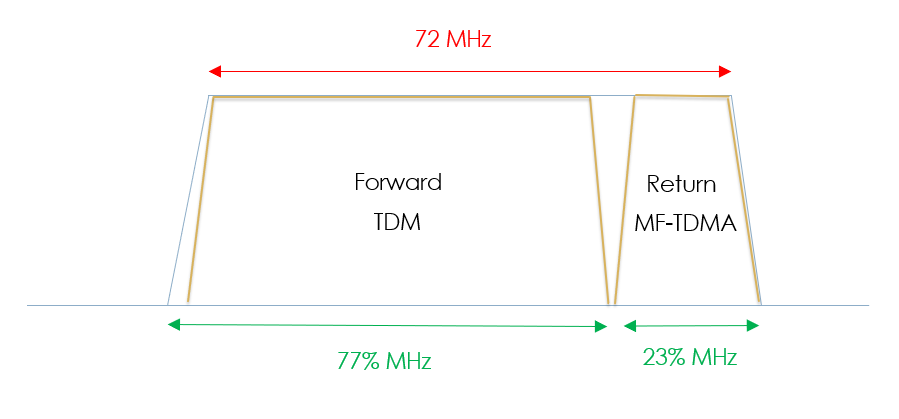
\includegraphics[width = .8\textwidth]{Transponder.png}
\caption{Representation of a transponder}
\label{fig:transp}
\end{figure}

Through these values the total number of transponder we have on the satellite is 12, 6 with horizontal polarization and 6 with the vertical one.

\subsection{Frequency Plan}
After these considerations the structure of the Frequency Plan is automatically elaborated and here it is represented in \autoref{fig:freqPlan}

\begin{figure}
\centering
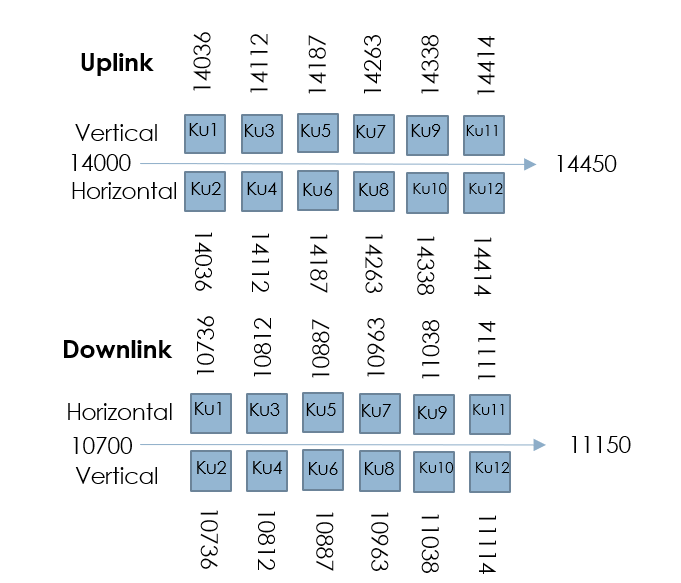
\includegraphics[width = .65\textwidth]{Frequencies.png}
\caption{Frequency plan for the communication module}
\label{fig:freqPlan}
\end{figure}

\subsection{Payload}
%% Definition of blocks:
\tikzset{%
  block/.style    = {draw, thick, rectangle, minimum height = 3em,
    minimum width = 3em},
	rect/.style    = {draw, thick, rectangle, minimum height = 3em,
	    minimum width = 1.5em},
	mux/.style    = {draw, thick, rectangle, minimum height = 7em,
			minimum width = 2.5em, align=left},
	triang/.style    = {draw, thick, isosceles triangle, minimum height = 3em, minimum width = 1.5em, align=left},
  mult/.style      = {draw, circle, node distance = 2.7cm},
  ghost/.style    = {coordinate}, % Input
  output/.style   = {coordinate} % Output
}
% Defining string as labels of certain blocks.
\newcommand{\mult}{\Large$\times$}
\newcommand{\inte}{$\displaystyle \int$}
\newcommand{\derv}{\huge$\frac{d}{dt}$}

\begin{tikzpicture}[auto, thick, node distance=2cm, >=triangle 45]
\draw
	% Drawing the blocks of first filter :
	node at (0,0)[right=-3mm, , label={below:(0)}]{\Large \textopenbullet}
	node [ghost, name=input1] {}
	% node [sum, right of=input1] (suma1) {\suma}
	node [rect, right of=input1, label={below:(1)}] (pol_sep) {}
  node [triang, right of=pol_sep, label={below:(2)}] (lna) {LNA}
  node [mult, right of=lna, label={D/C}, label={below:(3)}] (dlc) {\mult}
	node [triang, right of=dlc, label={below:(4)}] (ifa) {IF \\ amp}
	node [mult, right of=ifa, label={U/C}, label={below:(5)}] (ulc) {\mult}
	node [triang, right of=ulc, label={below:(6)}] (hpa) {HPA}
	node [triang, right of=hpa, label={below:(7)}] (bpf) {}
	node [mux, right of=bpf] (imux) {I \\M \\U \\ X}
	node at (19,1.5)[right=-3mm, name = ch1, label={left:$ch_1$}]{\Large \textopenbullet}
	node at (19,1)[right=-3mm, name = ch2]{}
	node at (19,0.5)[right=-3mm, name = ch3]{}
	node at (19,0)[right=-3mm, name = ch4]{}
	node at (19,-1.5)[right=-3mm, name = chN, , label={left:$ch_N$}]{}
	node [triang, right of=ch1, label={below:(8)}] (ca) {}
	node [block, right of=ca, label={below:(9)}] (alc) {ALC}
	node [triang, right of=alc, label={below:(10)}] (outamp) {}
	node [mux, right of=imux, node distance = 10cm] (omux) {O \\M \\U \\ X}
	node [triang, right of=omux, label={below:(11)}] (bpf2) {}
	node at (32,0)[right=-3mm, name = outantenna, label={below:(12)}]{\Large \textopenbullet};
    % Joining blocks.
    % Commands \draw with options like [->] must be written individually
	\draw[-](input1) -- node {}(pol_sep);
	\draw[-](pol_sep) -- node {} (lna);
	\draw[-](lna) -- node {$f_D$} (dlc);
	\draw[-](dlc) -- node {$f_{IF}$} (ifa);
	\draw[-](ifa) -- node {$f_{IF}$} (ulc);
	\draw[-](ulc) -- node {$f_u$} (hpa);
	% \draw[-](rx) -- node {} (bpf);
	\draw[-](hpa) -- node {} (bpf);
	\draw[-](bpf) -- node {} (imux);
	\draw[-](imux) -- node {} (ch1);
	\draw[-](imux) -- node {} (ch2);
	\draw[dashed](imux) -- node {} (ch3);
	\draw[dashed](imux) -- node {} (ch4);
	\draw[-](imux) -- node {} (chN);
	\draw[-](ch1) -- node {} (ca);
	\draw[-](ca) -- node {} (alc);
	\draw[-](alc) -- node {} (outamp);
	\draw[-](outamp) -- node {} (omux);
	\draw[-](omux) -- node {} (bpf2);
	\draw[-](bpf2) -- node {} (outantenna);

% 	% Boxing and labelling
	\draw [color=gray, dashed, label={Receiver Block}](1,-1.5) rectangle (14.5,1.5);
	\node at (6.5,1.5) [above=5mm, right=0mm] {\textsc{Receiver Block}};

	\draw [color=gray, dashed, label={Receiver Block}](14.8,2.5) rectangle (31,-2.5);
	\node at (21.5,2.5) [above=5mm, right=0mm] {\textsc{Repeater Block}};
	\draw [color=gray,thick](-0.5,-9) rectangle (12.5,-5);
	\node at (-0.5,-9) [below=5mm, right=0mm] {\textsc{second-order noise shaper}};
\end{tikzpicture}
The electronic part of the payload is composed by the two main sections of the \textbf{receiver block} and \textbf{repeater block}: in the first part, the signal is received, separated in polarization, filtered and amplified so as to be ready for the repeater part, in which it is channelized and further amplified. \autoref{fig:payload} shows the global representation of the payload.


\subsubsection{Receiver Block}
The main actions in which this block is involved are the \textbf{polarization separation} and the \textbf{frequency conversion}; \autoref{fig:receiver} shows accurately all the fundamental components of this first part.
\begin{itemize}
\item (1) is the polarization diplexer, which has the role of separating the received signal depending of its polarization; \autoref{fig:receiver} only shows the path for one possible polarization, but in the complete payload scheme all the components that follow the diplexer have to be doubled up;
\item (2) is a low noise amplifier necessary for a first recovering of the received signal; this amplifier is the main element which determines the figure of merit G/T of the transponder and thus it must have a low noise temperature (in this case is estimated of 438,45 K with a noise figure of 4 dB) and a high gain (in this case of 30 dB) in order to limit the role of the noise of subsequent stages.
\begin{sidewaysfigure}
\centering
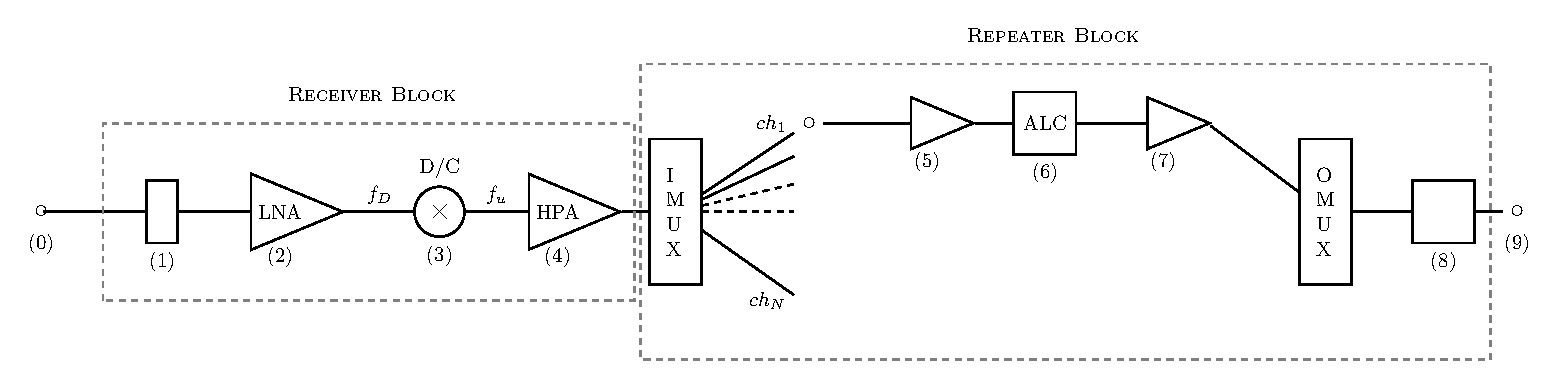
\includegraphics[width = 1\textwidth]{payload.pdf}
\caption{Payload representation}
\label{fig:payload}
\end{sidewaysfigure}
\item (3) is the frequency oscillator: its values change with respect to the frequency we need to convert, as shown in \autoref{tab:oscillator}. For the oscillator we have to monitor also other parameters like the conversion losses (normally in the order of 5 - 10 dB, we supposed the worst case of 10 dB and so a noise temperature of 2610 K) and the stability of the frequency \cite{Maral2017};
\item (4) is the High Power Amplifier necessary to amplify the converted signal before being channelized in the repeater section;
\item we also have to consider the role of the cables and the losses they bring inside the estimations; in our case we supposed a loss due to the cables of about 3 dB and an associate noise temperature of 288.63 K.
\end{itemize}
	\begin{table}
	\centering
	\begin{tabular}{lr}
	\toprule
	Downlink frequency & Oscillator frequency\\
	\midrule
	$10.95 \leq f_d \leq 11.2$ GHz & $1.5$ GHz\\
	$11.54 \leq f_d \leq 11.7$ GHz & $2.58$ GHz\\
	$12.5 \leq f_d \leq 12.75$ GHz & $3.8$ GHz\\
	\bottomrule
	\end{tabular}
	\caption{Oscillator frequency values depending of the Downlink frequency needed for an uplink frequency between 14 and 14.5 GHz}
	\label{tab:oscillator}
\end{table}
\begin{figure}[h]
	\centering
	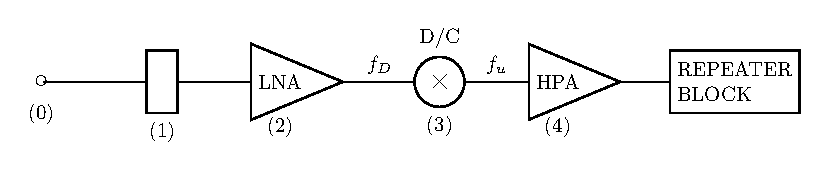
\includegraphics[width = \textwidth]{payload_receiver.pdf}
	\caption{Payload receiver part}
	\label{fig:receiver}
\end{figure}
For this block the redundancy is of 1/2.

\subsubsection{Repeater Block}
	In the repeater block the channelization part is present and, for that, the input/output multiplexers are needed. We selected 2 input and 2 output multiplexers, each one having 3 channels in order to have one channel per carrier received\footnote{we remember that the path described here is still referring to one single polarization. At the end of the description, all the elements described have to be doubled up in number}. Inside the multiplexers the main elements are the band-pass filters and the circulators used to separate the frequency channels, these ones are the main cause of losses inside the multiplexers since they depend on the number of times the signal concerned passes through a circulator (the loss is in the order of 0.1 dB).

In addition to this, for each channel of the multiplexers we then have:
	\begin{itemize}
	\item (5), a channel amplifier;
	\item (6), an Automatic Level Control module: a device needed to guarantee a constant power value as input of (7);
	\item (7), the amplifier module, composed by the EPS and the TWT sections which together form the Travelling Wave Tube Amplifier (TWTA). The output power value that we supposed for the TWTA section is 20W \cite{Maral2017}.
	\end{itemize}
	\begin{figure}[h]
		\centering
		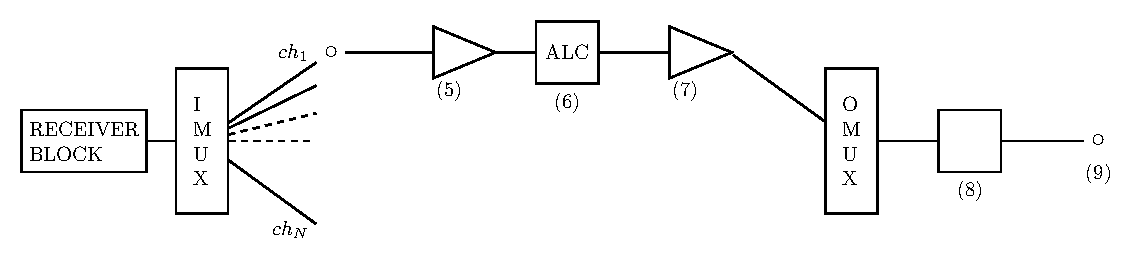
\includegraphics[width = \textwidth]{payload_repeater.pdf}
		\caption{Payload repeater part}
		\label{fig:repeater}
	\end{figure}
For this block the redundancy is a 8/12 redundancy ring.

\subsection{Power Budget}
The power budget mainly depends on the power required by the TWTA amplifiers in order to transmit the signal to the Earth. As can be seen from the chart in \autoref{fig:powerDistr}, the fraction of power that the communication subsystem requires is about 75 \%, all the other utilities uniformly share the remaining power needed.
\begin{figure}[h]
\centering
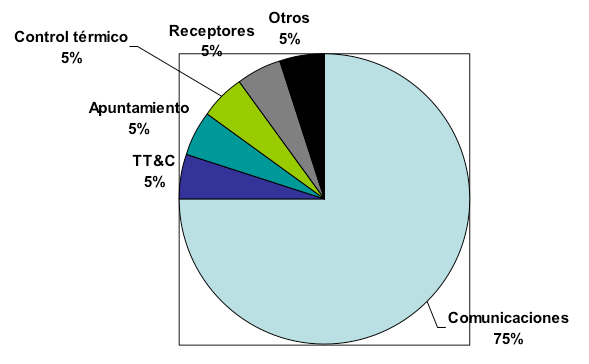
\includegraphics[width = .7\textwidth]{powerDistr.png}
\caption{Power distribution among the subsystems in percentage}
\label{fig:powerDistr}
\end{figure}
\subsubsection{Required Power}
	To estimate the required power we supposed to be in the worst case (end of life of the satellite) and followed the steps below:
\begin{itemize}
\item Estimate the \gls{eol} efficiency for the solar panel;
\item Estimate the \gls{eol} efficiency for the TWTA module;
\item Estimate the \gls{eol} efficiency for the EPC module;
\item Estimate the total power required for the transponders;
\item Estimate the total power required for the system;
\end{itemize}
\begin{description}
\item[Solar panel efficiency] Given an expected life of 15 years, a degrading coefficient $\frac{1}{\tau}$ of $0.043$ 1/s and an initial efficiency of 17 \%, the \gls{eol} solar panel efficiency is:
\begin{equation}
	\eta_{SP_{EOL}} = \eta_{BOL}e^{-0.043T} \rightarrow \eta_{SP_{EOL}} = \frac{17}{100}e^{-0.043\times 15} = 8.9 \%
\end{equation}
\item[TWT efficiency] The same expression can be used to estimate the \gls{eol} efficiency for the TWTA, supposing a $\eta_{TW_{BOL}} = 60\%$: in particular, if we suppose that the efficiency value will be reduced of 10\% after 10 years (6\% of decrement), we can find the degradation coefficient $\frac{1}{\tau}$ as:
\begin{equation}
60 \% - 6 \% =60 \% e^{\frac{-10}{\tau}} \rightarrow \tau = \frac{-10}{log_e\frac{54}{60}} = 94.91 \quad s^{-1}
\end{equation}
and so the \gls{eol} efficiency:
\begin{equation}
\eta_{TW_{EOL}} = 60e^{\frac{-15}{94.91}} = 51.23 \%
\end{equation}
\item[EPC efficiency] Through the same procedure we obtain also the efficiency for the EPC segment:
\begin{equation}
\eta_{EPC_{EOL}} = 81.2 \%
\end{equation}
\item[Total power required for the transponders] With all the efficiency values previously found we can now estimate the total power used by the satellite in the worst case, supposing an output power at saturation for the TWT module of 250 W:
\begin{align}
P_{in_{TW}} &= \frac{P_{out_{TW}}}{\eta_{TW_{EOL}}} = 195.198 \text{ W}\\
P_{in_{EPC}} &= \frac{P_{in_{TW}}}{\eta_{EPC_{EOL}}} = 240.39 \text{ W}\\
P_{transp} &= P_{in_{EPC}} \times N_{transp} = 240.39 \times 12 = 2.885 \text{ kW}\\
\end{align}
Moreover, since this power consists in the 75\% of the total power necessary for the satellite, the total power for the satellite is:
\begin{equation}
P_{tot} = \frac{P_{transp}}{75\%} = 3.846 \text{ kW}
\end{equation}
\end{description}
\subsubsection{Solar Panels specifications}
	Once we have found the total power that the satellite needs at the worst case, the estimation of the area for the solar panels is made deploying the following expression:
\begin{equation}
A_{panel} = \frac{P_{tot} s}{f \Phi \eta_{SP_{EOL}} s (1 - l)}
\end{equation}
Where:
\begin{itemize}
\item $s$ is the area of a single cell;
\item $\Phi$ is the solar flux, supposed to be of 1215,74 $W/m^2$ in the farthest point of the satellite orbit (based on the observation of \autoref{fig:flux});
\item $f$ is the filling efficiency, here of the order of 90 \%;
\item $l$ are general losses due to cabling and cover and typical values are 10 to 15 \% (here we selected 15 \% for a worst-case analysis);
\end{itemize}
\begin{figure}[h]
\centering
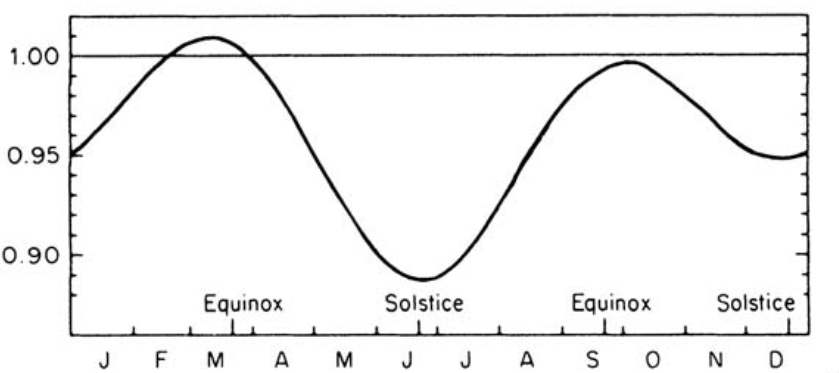
\includegraphics[width = .7\textwidth]{flux.png}
\caption{Combined influence of sun declination and distance variation}
\label{fig:flux}
\end{figure}
And from it the final value for the solar panel area of our satellite is:
\begin{equation}
A = 46.46 \text{ $m^2$}
\end{equation}
\subsection{Weight Estimation}
\lipsum[1]
